\documentclass[oneside]{thesisclass}
% Based on thesisclass.cls of Timo Rohrberg, 2009
% ----------------------------------------------------------------
% Thesis - Main document
% ----------------------------------------------------------------

\usepackage{floatflt}


%% -----------------------------
%% | Information for titlepage |
%% -----------------------------

\newcommand{\myname}{Jan Andre Rudolph}
\newcommand{\mytitle}{Matrices \& Mazes \\in Quantum Algorithms}
\newcommand{\semesterD}{Sommersemester 2017}
\newcommand{\semesterE}{Summer term 2017}


%%%%%%%%%%%%%%%%%%%%%%%%%%%%%%%%%
%% Here, main documents begins %%
%%%%%%%%%%%%%%%%%%%%%%%%%%%%%%%%%
\begin{document}

\selectlanguage{english}

\frontmatter
\pagenumbering{roman}
%% titlepage.tex
%%

% coordinates for the bg shape on the titlepage
\newcommand{\diameter}{20}
\newcommand{\xone}{-15}
\newcommand{\xtwo}{160}
\newcommand{\yone}{15}
\newcommand{\ytwo}{-253}

\begin{titlepage}
% bg shape
\begin{tikzpicture}[overlay]
\draw[color=gray]  
 		 (\xone mm, \yone mm)
  -- (\xtwo mm, \yone mm)
 arc (90:0:\diameter pt) 
  -- (\xtwo mm + \diameter pt , \ytwo mm) 
	-- (\xone mm + \diameter pt , \ytwo mm)
 arc (270:180:\diameter pt)
	-- (\xone mm, \yone mm);
\end{tikzpicture}
	\begin{textblock}{10}[0,0](4,2.5)
		
\includegraphics[width=.3\textwidth]{logos/KITLogo_RGB.pdf}
	\end{textblock}
	\changefont{phv}{m}{n}	% helvetica	
	\vspace*{3.5cm}
	\begin{center}
		\Huge{\mytitle}
		\vspace*{2cm}\\
		\Large{
			\iflanguage{english}{by} {von}
		}\\
		\vspace*{1cm}
		\huge{\myname}\\
		\vspace*{4cm}
		\Large{Seminar}\\
                \vspace{1cm}
		\huge{Quantum Algorithms}\\
		\Large{
                \vspace{1cm}
                \Large{Institute of Theoretical Informatics, KIT}\\
			\iflanguage{english}{\semesterE} {\semesterD}
                \vspace{1cm}
		}
	\end{center}
	\vspace*{1cm}

\vspace{2cm}

\begin{textblock}{10}[0,0](4,16.8)
\tiny{ 
	\iflanguage{english}
		{KIT -- University of the State of Baden-Wuerttemberg and National Research Center of the Helmholtz Association}
		{KIT -- Universit\"at des Landes Baden-W\"urttemberg und nationales Forschungszentrum in der Helmholtz-Gemeinschaft}
}
\end{textblock}

\begin{textblock}{10}[0,0](14,16.75)
\large{
	\textbf{www.kit.edu} 
}
\end{textblock}

\end{titlepage}

\definecolor{kit-green50}{rgb}{.50,.79,.75}


%% -------------------
%% |   Directories   |
%% -------------------
\tableofcontents


%% -----------------
%% |   Main part   |
%% -----------------
\mainmatter
\pagenumbering{arabic}
\chapter{Introduction}
\nocite{*}
The operationality of Quantum Computers will progress quickly in the next years. 
When Moores Law reaches the "firewall" of atom physics, the quantum physics will lead us to a new kind of information, carried by the so-called q-bits. 
Therefore the importance of understanding quantum algorithms rises. 
All computer scientists should at least be aware of the possibilities quantum algorithms provide, because the work of today may be affected by quantum computing in the near future. \\
\\There is not yet a high level quantum coding language that compiles in some sense, but we have three basic options to represent quantum operations.
There are so called quantum circuits that just represent the physical structure. 
But unlike electronic circuits, these are very complicated to interpret.
Due to the quantum entanglement, one cannot linearly read the circuit. 
Merely one has to understand the whole circuit at once, including all measurement. 
If we do not want to understand the complete circuit before we understand one part of it, we can use linear algebra. \\
\\We will see that we can use matrices to represent circuits or smaller modules of it. 
Not only that mathematics is a global language with the advantages of provability and that computers understand it.
But we will also see that we now have the possibility to explicitly represent, calculate and understand quantum entanglement.
The only remaining problem (besides scalability) is that matrices do not provide a natural image nor the idea of what happens.\\
\\This is where the mazes as our third option of representation have their might.
The so called mazes are a graph based translation of the matrices just like adjacency matrices and the corresponding adjacency graphs - just a little more complicated.
We will introduce some mice as a guide through the mazes and as an anchor for the imagination.\\
\\This thesis aims to briefly explain the concepts of matrices and mazes and connects them to the idea of circuits. 
Some important matrices for quantum algorithms will be introduced and explained - also by the use of mazes.
The text is mainly inspired by the book Quantum Algorithms via Linear Algebra from R.J.Lipton and K.W.Regan.
It may target any kind of computer scientists or persons with an equal level of mathematics and technology.\\

\chapter{Linear Algebra}
%\section{Hilbert Space}
Before we can talk about matrices, we need to consider the role of vectors and matrices in the model.
To understand the Hilbert space we are moving in, it seems a good first step to have a look at the Euclidean space.
The Euclidean space is in general n-dimensional.
Normally one describes geometrical objects as subsets of the space, where vectors correspond to points.
With the inner product, the Euclidean space provides the possibility to measure angles and distances.
To represent quantum states, we need complex numbers and therefore the Hilbert space.
The scalar product and the transposition now need the complex conjugated of the imaginary numbers but in general the operations are the same.\\
\\To represent an algorithm we now use a vector as input.
We multiply one or more of our matrices on the left side and the result is again a vector.
This vector represents the output.\\

\section{Feasibility}
But we cannot build just any matrix in an actual quantum circuit.
Or in other words not all matrices are quantum feasible.
To determine which matrices are feasible, we kind of translate the definition of feasibility for quantum circuits.
Intuitively we call a circuit quantum feasible if we only have to spend a polynomial growing amount of resources when the complexity grows linearly.
This way we can support a polynomial amount of gates and a polynomial amount of lanes.
Translating it into the terms of linear algebra, we must therefore assume some kind of basic matrices to substitute physical gates.
Those basic matrices are no elementary matrices and elementary matrices are no basic matrices neither.
Still, this does not mean a disjunction.
Basic matrices mean the corresponding matrices to gates we can physically build.
So a basic matrix $\mathbf B$ can be any unitary matrix $\mathbf U \in d \times d$ where d is constant and we can use some tensor product with the identity matrix to enlarge the basic matrix with ones on the expanded diagonal.
This basic matrix is feasible.
Now we can set up a whole feasible computation $\mathbf C = \mathbf F_t...\mathbf F_1\mathbf F_0$.
$F_i$ must be feasible, e.g. a basic matrix $\mathbf B$, it must be of polynomial order and t must be polynomial, too.\\

\chapter{Boolean Functions}
The first class of matrices are those representing Boolean functions.
Actually those matrices do not represent the functions directly, but we will need some boundary conditions to succeed.
These conditions must predefine how to interpret the input and output vector.
But not all Boolean functions are quantum feasible and for some it is not yet clear.
Au contraire, one can think of some complicated Boolean functions which will not be quantum feasible.
So in the following sections there will be some matrices introduced.
Then we will link it up to the concept of Boolean functions.
All those matrices have in common, that they are built of only ones and zeros.
So the mazes look just like connectivity graphs. 
That means that we do not need all the 'features' of mazes yet.
Another common point of all these matrices is that the unitarity falls directly out of the fact, that the matrices' column vectors obviously build a standard basis.\\

\section{SWAP}
The most trivial kind of matrices is the Identity - this means that the input equals the output.
Obviously this is a Boolean function - but not the most interesting one.
If we now swap the columns in the middle as shown in figure \ref{swap} we have to look at the binary strings to understand what physically happens.

\begin{figure}
\begin{center}
  $
 \begin{pmatrix}
  1 & 0 & 0 & 0 \\
  0 & 0 & 1 & 0 \\
  0 & 1 & 0 & 0 \\
  0 & 0 & 0 & 1
  \end{pmatrix}
 $
 \caption{SWAP}
 \label{swap}
 \end{center}
\end{figure}

For no input or input on both lanes, the behaviour equals the identity.
But if there is only input on one lane, the '1' in the SWAP matrix connects the binary strings to their inverse.
And this is just what the corresponding maze \ref{swapM} shows us - the edges connects the input node '01' with the output node '10' as well as '10' with '01'.
\begin{figure}
\begin{center}
  \begin{tikzpicture}
   [scale=.4,auto=left,every node/.style={circle,fill=kit-green50}]
   \node (n00r) at (12,6)  {00};
   \node (n00m) at (6,6)  {00};
   \node (n01r) at (12,4)  {01};
   \node (n01m) at (6,4)  {01};
   \node (n10r) at (12,2)  {10};
   \node (n10m) at (6,2)  {10};
   \node (n11r) at (12,0)  {11};
   \node (n11m) at (6,0)  {11};
   \foreach \from/\to in {n00m/n00r,n01m/n10r,n10m/n01r,n11m/n11r}
    \draw[thick] (\from) -- (\to);
   \end{tikzpicture}
   \caption{SWAP}
   \label{swapM}
   \end{center}
\end{figure}

So in general this matrix swaps the two lanes.
A SWAP matrix is a basic matrix and therefore obviously feasible.\\

\section{CNOT}
Due to the superpositioning, the behaviour heavily changes if we choose to swap two other columns as shown in figure \ref{cnot} as matrix - the CNOT matrix - and in figure \ref{cnotM} as a maze.
\begin{figure}
\begin{center}
 $
 \begin{pmatrix}
  1 & 0 & 0 & 0 \\
  0 & 1 & 0 & 0 \\
  0 & 0 & 0 & 1 \\
  0 & 0 & 1 & 0
  \end{pmatrix}
 $
  \caption{CNOT}
  \label{cnot}
  \end{center}
\end{figure}
\begin{figure}
\begin{center}
  \begin{tikzpicture}
   [scale=.4,auto=left,every node/.style={circle,fill=kit-green50}]
   \node (n00m) at (6,6)  {00};
   \node (n00l) at (0,6)  {00};
   \node (n01m) at (6,4)  {01};
   \node (n01l) at (0,4)  {01};
   \node (n10m) at (6,2)  {10};
   \node (n10l) at (0,2)  {10};
   \node (n11m) at (6,0)  {11};
   \node (n11l) at (0,0)  {11};
   %CNOT
   \foreach \from/\to in {n00l/n00m,n01l/n01m,n11l/n10m,n10l/n11m}
    \draw[thick] (\from) -- (\to);
   \end{tikzpicture}
   \caption{CNOT}
   \label{cnotM}
   \end{center}
\end{figure}


CNOT stands for controlled not - what intuitively toggles the second, physical lane if the first is one.
As we can easily read in the maze, the second lane - the LSB in the Boolean string - is toggled when and only when the first lane - the MSB in the Boolean string - is one.\\
\\As already mentioned, we can use this behaviour to implement some Boolean functions.
The general procedure is described in the following for the XOR function as an example.\\
\\Since we cannot change the behaviour of the CNOT gate, we have to find a convention for the in- and output that fits the desired function.
We need both lanes as input and one of the two output lanes that is interpreted as the result.
Referring to the maze again, we can just try out both lanes.
If we choose the first lane, the output for XOR(0,1) would be 0 since '01' is connected to '01' where 0 is on the first lane.
This obviously does not match the XOR function.
But for the second lane regarded as output, we obtain the results we expected.\\
\\Another example is the NOT function - which only takes one input lane.
Looking at the maze, we directly see that the second lane is toggled when the first lane is '1'.
This is what we want to achieve - so we set the first lane '1' and regard the second lane as in- and output.
This way the input is always toggled.\\

\section{Toffoli Gate}
If we extend the CNOT gate by another (physical) control lane we call it CCNOT - controlled controlled not - also known as Toffoli gate.
This gate has three lanes.
Therefore, the corresponding matrix, as well as the maze, displays $2^3$ superpositions.
So it is of order 8.
Looking at the matrix \ref{tof} it might not be intuitive where the 'controlled controlled' comes from.
\begin{figure}
 \begin{center}
  $
  \begin{pmatrix}
  1 & 0 & 0 & 0 & 0 & 0 & 0 & 0 \\
  0 & 1 & 0 & 0 & 0 & 0 & 0 & 0 \\
  0 & 0 & 1 & 0 & 0 & 0 & 0 & 0 \\
  0 & 0 & 0 & 1 & 0 & 0 & 0 & 0 \\
  0 & 0 & 0 & 0 & 1 & 0 & 0 & 0 \\
  0 & 0 & 0 & 0 & 0 & 1 & 0 & 0 \\
  0 & 0 & 0 & 0 & 0 & 0 & 0 & 1 \\
  0 & 0 & 0 & 0 & 0 & 0 & 1 & 0
  \end{pmatrix}
  $
  \caption{Toffoli Gate}
  \label{tof}
 \end{center}
\end{figure}
But again, the maze \ref{tofM} is more clear, even if it is already quite big. 
\begin{figure}
 \begin{center}
  \begin{tikzpicture}
   [scale=.4,auto=left,every node/.style={circle,fill=kit-green50,inner sep=0}]
   \node (n000r) at (6,14)  {000};
   \node (n000l) at (0,14)  {000};
   \node (n001r) at (6,12)  {001};
   \node (n001l) at (0,12)  {001};
   \node (n010r) at (6,10)  {010};
   \node (n010l) at (0,10)  {010};
   \node (n011r) at (6,8)  {011};
   \node (n011l) at (0,8)  {011};
   \node (n100r) at (6,6)  {100};
   \node (n100l) at (0,6)  {100};
   \node (n101r) at (6,4)  {101};
   \node (n101l) at (0,4)  {101};
   \node (n110r) at (6,2)  {110};
   \node (n110l) at (0,2)  {110};
   \node (n111r) at (6,0)  {111};
   \node (n111l) at (0,0)  {111};
   \foreach \from/\to in {n000l/n000r,n001l/n001r,n010l/n010r,n011l/n011r,n100l/n100r,n101l/n101r,n110l/n111r,n111l/n110r}
    \draw[thick] (\from) -- (\to);
  \end{tikzpicture}
  \caption{Toffoli Gate}
  \label{tofM}
 \end{center}
\end{figure}
All nodes are connected to their identity, only the last two are toggled.
In other words, if you look at the Boolean strings of these nodes the input of the last physical lane is toggled when and only when the first two lanes are one.\\
\\With Toffoli gates one can build any Boolean function. 
It is called a universal Boolean gate.
As a first example we will construct an AND function.
This uses only one Toffoli gate, so we can just think about the boundary conditions like before.
The AND function requires two input lanes and one output lane.
The output lane shall be one if and only if both input lanes are one.
Looking at the maze \ref{tofAnd}, we see that the MSB of the Boolean string is toggled when and only when both other lanes are one.
\begin{figure}
 \begin{center}
  \begin{tikzpicture}
   [scale=.4,auto=left,every node/.style={circle,fill=kit-green50,inner sep=0}]
   \node (n000r) at (6,14)  {00\textbf{0}};
   \node (n000l) at (0,14)  {\textbf{00}0};
   \node (n010r) at (6,10)  {01\textbf{0}};
   \node (n010l) at (0,10)  {\textbf{01}0};
   \node (n100r) at (6,6)  {10\textbf{0}};
   \node (n100l) at (0,6)  {\textbf{10}0};
   \node (n111r) at (6,0)  {11\textbf{1}};
   \node (n110l) at (0,2)  {\textbf{11}0};
   \foreach \from/\to in {n000l/n000r,n010l/n010r,n100l/n100r,n110l/n111r}
    \draw[thick] (\from) -- (\to);
   %GRAY
   \node[fill=lightgray] (n001r) at (6,12)  {001};
   \node[fill=lightgray] (n001l) at (0,12)  {001};
   \node[fill=lightgray] (n011r) at (6,8)  {011};
   \node[fill=lightgray] (n011l) at (0,8)  {011};
   \node[fill=lightgray] (n101r) at (6,4)  {101};
   \node[fill=lightgray] (n101l) at (0,4)  {101};
   \node[fill=lightgray] (n110r) at (6,2)  {110};
   \node[fill=lightgray] (n111l) at (0,0)  {111};
   \foreach \from/\to in {n001l/n001r,n011l/n011r,n101l/n101r,n111l/n110r}
    \draw[color=gray,thick] (\from) -- (\to);
  \end{tikzpicture}
  \caption{Toffoli Gate}
  \label{tofAnd}
 \end{center}
\end{figure}
This is already quite similar to the behaviour of AND.
We can now set this last lane zero and we finally generated the desired behaviour.
On output lane 3 we measure one if and only if both input lanes - lane '1' and '2' - are set to one.\\
\\The physical circuit, figure \ref{andP}, looks way more compact.
\begin{figure}
 \begin{center}
  \begin{tikzpicture}
   [scale=1,auto=left,every node/.style={circle,fill=kit-green50}]
   \node (n3) at (0,1) {"0"};
   \node (n2) at (0,3) {in$_2$};
   \node (n1) at (0,4) {in$_1$};
   \node (n0) at (4,1) {out};
   \draw[thick] (n3) -- (n0);
   \draw[thick] (n2) -- (4,3);
   \draw[thick] (n1) -- (4,4);
   \draw[thick] (2,4) -- (2,0.75);
   \draw (2,1) circle (0.25);
   \draw[fill=black] (2,3) circle (0.15);
   \draw[fill=black] (2,4) circle (0.15);
  \end{tikzpicture}
  \caption{Toffoli Gate}
  \label{andP}
 \end{center}
\end{figure}
On the left-hand side we find the input lanes '1' and '2' as well as the third lane which is constantly set to zero.
Previously these lanes were implicitly represented in the Boolean strings, but now they are pictured as nodes in the graph.
The same goes for the output, where the first two lanes are not connected to anything since we noticed that we only need the third output lane.\\
\\Now look at the last step again - with Boolean universality in mind.
If we set the last lane one instead of zero, we get a NAND.
The one on the last lane is toggled to zero if and only if the two first lanes - our input lanes - are one.
Since the NAND is universal for Boolean functions, we finally argumented why the Toffoli gate is universal for Boolean functions.\\

\section{Controlled M}
There is another important gate which is universal for Boolean functions.
If we do not control the NOT like the CNOT and neither control the CNOT like the CCNOT but control the SWAP from the beginning - we get a C-SWAP \ref{fred}.
\begin{figure}
 \begin{center}
  \begin{tikzpicture}
   [scale=.4,auto=left,every node/.style={circle,fill=kit-green50,inner sep=0}]
   \node (n000r) at (6,14)  {000};
   \node (n000l) at (0,14)  {000};
   \node (n001r) at (6,12)  {001};
   \node (n001l) at (0,12)  {001};
   \node (n010r) at (6,10)  {010};
   \node (n010l) at (0,10)  {010};
   \node (n011r) at (6,8)  {011};
   \node (n011l) at (0,8)  {011};
   \node (n100r) at (6,6)  {100};
   \node (n100l) at (0,6)  {100};
   \node (n101r) at (6,4)  {101};
   \node (n101l) at (0,4)  {101};
   \node (n110r) at (6,2)  {110};
   \node (n110l) at (0,2)  {110};
   \node (n111r) at (6,0)  {111};
   \node (n111l) at (0,0)  {111};
   \foreach \from/\to in {n000l/n000r,n001l/n001r,n010l/n010r,n011l/n011r,n100l/n100r,n101l/n110r,n110l/n101r,n111l/n111r}
    \draw[thick] (\from) -- (\to);
  \end{tikzpicture}
  \caption{Fredkin Gate}
  \label{fred}
 \end{center}
\end{figure}
This C-SWAP is also called Fredkin gate - and is the first universal gate that was actually built in a laboratory.
Nomen est omen, it works just like the CCNOT.
The two last lanes are swapped if the first is one.
Since we discussed the Toffoli gate well, we do not need to go into details again.\\
\\But what we can do is generalizing the 'controlled' matrices.
Unfortunately - or fortunately? - this also applies to non-Boolean functions, so technically it does not belong to this chapter.
The idea is, that we have seen some matrices that we can control.
And now we can consider that we can control any feasible matrix.
Comparing the mazes we see that they have in common that the output is the identity when the LSB in the Boolean string is zero.
On the other hand when the LSB in the Boolean string is one, the output is the controlled matrix.
Naturally the LSB is zero for exactly the first/upper half of the lines.
So the Controlled-M matrix has the Identity in the upper left and the $\mathbf M$ in the down right-hand side.
This is shown in figure \ref{cm} for some unknown, but by definition feasible, matrix $\mathbf M_k$.
It scales for any order k that equals some power of two.
\begin{figure}
 \begin{center}
  $
 \begin{pmatrix}
  \mathbf I_k & \mathbf 0_k \\
  \mathbf 0_k & \mathbf M_k
  \end{pmatrix}
 $
  \caption{Controlled-M}
  \label{cm}
 \end{center}
\end{figure}

\chapter{Hadamard Matrix}
Having discussed Boolean functions, we can now take the next step.
Hadamard matrices aim to have the maximum possible determinant while being filled with only plus and minus '1' - and being orthogonal.
The orthogonality is important at this point since we need unitary matrices for our quantum algorithms.
Unfortunately, it is not proven that those matrices exist for every order.
For most orders, it is even proven that there exists an upper boundary for the determinant of Hadamard matrices - if such exist - that is unequal smaller than the square root of the order.
The general upper bound for the Hadamard matrices determinant is the square root of the order.
Luckily we can easily find Hadamard matrices that fulfill this upper bound - if we limit to orders equal some power of two.
These special matrices are also called Sylvester matrices.
While defining this general Hadamard matrix recursively, we can parallely prove feasibility.\\
\\Initially we take the matrix of order two which is shown in figure \ref{h2}
which is a Hadamard matrix for the following two reasons.
\begin{figure}
 \begin{center}
  $
 \begin{pmatrix}
  \mathbf 1 & \mathbf 1 \\
  \mathbf 1 & \mathbf -1
  \end{pmatrix}
 $
  \caption{$\mathbf H_2$}
  \label{h2}
 \end{center}
\end{figure}
The two column or row vectors are obviously orthogonal, therefore they build a standard basis - so the matrix is orthogonal.
The absolute determinant $d_2$ is defined by $d_2 = |\mathbf H_{11} * \mathbf H_{22} - \mathbf H_{12} * \mathbf H_{21}| = |1 * (-1) - 1 * 1| = |(-2)| = 2$ which as we remember reaches the upper bound.
By Tensoring the outer product of this $\mathbf H_2$ Hadamard matrix with itself, we gain the $\mathbf H_4$ matrix of order 4 which is again a Haramard matrix.
This tensoring with $\mathbf H_2$ can be continued until the order equals any power of two.
So we only use a tensor product and the basic $\mathbf H_2$ matrix, what provides us feasibility.\\
\\Unlike the matrices for Boolean functions, we now need to additionally normalize the matrix.
Strictly speaking, this is not nessecary for Hadamard matrices, but for quantum algorithms since we need unitary matrices.
Therefore, not a normal matrix is meant but a matrix whose column-vectors are normalized.
Also Sylvester matrices are orthogonal by definition - you can intuitively see how the outer product with $\mathbf H_2$ is responsible for this.
This is not a real problem and we will not explicitly do that in the following, but in general you can see it in the graphics.
The normalization is solved by simply deviding the matrix by the square root of the order.
We have already seen that this is the determinant of those Hadamard matrices we are regarding.\\
\\The corresponding maze \ref{h4}
now has negative edges.
\begin{figure}
 \begin{center}
  $
 \begin{pmatrix}
  1 & 1 & 1 & 1 \\
  1 & -1 & 1 & -1 \\
  1 & 1 & -1 & -1 \\
  1 & -1 & -1 & 1
  \end{pmatrix}
 $
  \caption{$\mathbf H_4$}
  \label{h4}
 \end{center}
\end{figure}
In the following, those are represented by dashed lines.
Also in the Boolean mazes we had only one path while we now see many edges going in and out the nodes.
Therefore, we shall first ensure how to read this.
We pick two nodes, one from the left side and one from the right side.
Following one path from the left side to the right side, all edge-weights are multiplied - but in this case all paths are of length one.
Then in the most right nodes, all incoming, multiplied weights are summed up - but in this case also only one path connects two nodes.
At least they are divided by the normalization factor.
We will soon see deeper mazes.
Multiplying a matrix on the left side translates to concatenating a maze on the right side.
It is interesting to see what happens if we concatenate another Hadamard matrix.
Since it is its own transpose, or respectively as a unitary matrix its own inverse, you gain back the identity.
In other words this means that the first Hadamard gate 'mixes' all your physical lanes, but the second Hadamard gate exactly 'un-mixes' it.\\

\chapter{Fourier Matrix}
The next degree of 'mixing' lanes does the Fourier matrix.
It introduces complex numbers - the reason why we chose the Hilbert space over the Euclidean space.
A first fun fact is, that $\mathbf F_2$ just equals $\mathbf H_2$. 
But now we will briefly discuss the definition which is way more involved.\\
\\First we need to recapitulate what is a root of unity.
The $n^{th}$ root of unity is defined by $\omega _n = e^{-2\pi i/n}$ or equivalently $\tilde{\omega} _n = e^{2\pi i/n}$.
It describes a point in the unit sphere that is turned by the angle of $1/n * 360^\circ$.
Figure \ref{root} illustrates this for $n = 8$.
\begin{figure}
 \begin{center}
  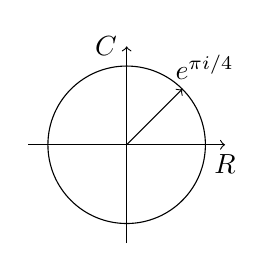
\begin{tikzpicture}
  \draw[->] (-1.25,0) -- (1.25,0) coordinate (X) node[below] {$\mathbb R$};
  \draw[->] (0,-1.25) -- (0,1.25) node[left] {$\mathbb C$};
  \newcommand\CircleRadius{1cm}
  \draw (0,0) circle (\CircleRadius);
  \coordinate (P) at (45:\CircleRadius);
  \node (pName) at (45:1.4) {$e^{\pi i/4}$};
  \draw[->] (0,0) -- (P);
\end{tikzpicture}
\caption{$\tilde{\omega} _8$}
\label{root}
 \end{center}
\end{figure}

So we need to multiply (/concatenate) n $n^{th}$ roots of unity to get back a real '1', respectively $w_n^n = 1$.
To build a Fourier matrix of order n, we put at position jk the $jk^{th}$ power of the $n^{th}$ root of unity, respectively $\mathbf F_n = \Big( \omega _{kj}^{kj}\Big)$.
For big exponents we can use the fact that by definition $\omega$ is a primitive root of unity, so we can use $\omega ^{x} = \omega ^{y} \iff x \equiv y \text{ mod}(n)$ to modulo the exponents \ref{fMod}.
\begin{figure}
 \begin{center}
  $
  \begin{pmatrix}
    \omega ^0 & \omega ^0 & \omega ^0 & \omega ^0 & \omega ^0 & \omega ^0 & \omega ^0 & \omega ^0 \\
    \omega ^0 & \omega ^1 & \omega ^2 & \omega ^3 & \omega ^4 & \omega ^5 & \omega ^6 & \omega ^7 \\
    \omega ^0 & \omega ^2 & \omega ^4 & \omega ^6 & \omega ^0 & \omega ^{2} & \omega ^{4} & \omega ^{6} \\
    \omega ^0 & \omega ^3 & \omega ^6 & \omega ^1 & \omega ^{4} & \omega ^{7} & \omega ^{2} & \omega ^{5} \\
    \omega ^0 & \omega ^4 & \omega ^0 & \omega ^{4} & \omega ^{0} & \omega ^{4} & \omega ^{0} & \omega ^{4} \\
    \omega ^0 & \omega ^5 & \omega ^{2} & \omega ^{7} & \omega ^{4} & \omega ^{1} & \omega ^{6} & \omega ^{3} \\
    \omega ^0 & \omega ^6 & \omega ^{4} & \omega ^{2} & \omega ^{0} & \omega ^{6} & \omega ^{4} & \omega ^{2} \\
    \omega ^0 & \omega ^7 & \omega ^{6} & \omega ^{5} & \omega ^{4} & \omega ^{3} & \omega ^{2} & \omega ^{1} 
  \end{pmatrix}
  $
  \caption{$\mathbf F_8$}
  \label{fMod}
 \end{center}
\end{figure}
\\In figure \ref{f8} we can see the same 8x8 Fourier matrix with simplifies entries.
\begin{figure}
 \begin{center}
  $
  \begin{pmatrix}
    1 & 1 & 1 & 1 & 1 & 1 & 1 & 1 \\
    1 & \omega & -i & -i\omega & -1 & -\omega & i & i\omega \\
    1 & -i & -1 & i & 1 & -i & -1 & i \\
    1 & -i\omega & i & \omega & -1 & i\omega & -i & -\omega \\
    1 & -1 & 1 & -1 & 1 & -1 & 1 & -1 \\
    1 & -\omega & -i & i\omega & -1 & \omega & i & -i\omega \\
    1 & i & -1 & -i & 1 & i & -1 & -1 \\
    1 & i\omega & i & -\omega & -1 & -i\omega & -i & \omega     
  \end{pmatrix}
  $
  \caption{$\mathbf F_8$}
  \label{f8}
 \end{center}
\end{figure}
There are positive and negative numbers, real and complex numbers involved - especially omega.
One can also represent omega in a maze, but I would not call that intuitive anymore because the calculations become too complex.\\
\\For Fourier matrices of order $n = 4$ the case is bit easier.
The reason is $\omega _4 = e^{-\pi i/2} = -i$ what means that there is no omega left if we simplify the terms, visualized in figure \ref{f4}.
\begin{figure}
 \begin{center}
  $
  \begin{pmatrix}
  1 & 1 & 1 & 1 \\
  1 & -i & -1 & i \\
  1 & -1 & 1 & -1 \\
  1 & i & -1 & -i
  \end{pmatrix}
  $
  \caption{$\mathbf F_4$}
  \label{f4}
 \end{center}
\end{figure}
The inverse can be understood in two ways.
The unitarity provides us that the conjugate transpose is the inverse.
But it is more helpful to remind the intuition of roots of unity.
Remember, $\tilde{\omega}$ is an equal root of unity - but it turns in the opposite direction on the unit sphere.
We call the corresponding Fourier matrix $\tilde{\mathbf F}$ \ref{fH}, which also equals the inverse.\\
 \begin{figure}
 \begin{center}
  $
  \begin{pmatrix}
  1 & 1 & 1 & 1 \\
  1 & i & -1 & -i \\
  1 & -1 & 1 & -1 \\
  1 & -i & -1 & i
  \end{pmatrix}
  $
  \caption{$\mathbf{\tilde F}_4$}
  \label{fH}
 \end{center}
\end{figure}
\\Before we can look at an example maze, we have to remember that the dashed edges equal negative numbers and now we introduce colored edges representing 'i'.
With that in mind we can carefully evaluate the maze in figure \ref{fM}, which represents the calculation $\mathbf F\tilde{\mathbf F} = \mathbf R$.
\begin{figure}
 \begin{center}
  \begin{tikzpicture}
   [scale=.4,auto=left,every node/.style={circle,fill=kit-green50}]
   \node (n00r) at (18,6)  {00};
   \node (n00m) at (9,6)  {00};
   \node (n00l) at (0,6)  {00};
   \node (n01r) at (18,4)  {01};
   \node (n01m) at (9,4)  {01};
   \node (n01l) at (0,4)  {01};
   \node (n10r) at (18,2)  {10};
   \node (n10m) at (9,2)  {10};
   \node (n10l) at (0,2)  {10};
   \node (n11r) at (18,0)  {11};
   \node (n11m) at (9,0)  {11};
   \node (n11l) at (0,0)  {11};
   %positive real left
   \foreach \from/\to in {n00l/n00m,n00l/n01m,n00l/n10m,n00l/n11m,n01l/n00m,n10l/n00m,n11l/n00m,n10l/n10m}
    \draw[thick] (\from) -- (\to);
   %negative real left
   \foreach \from/\to in {n10l/n01m,n01l/n10m,n11l/n10m,n10l/n11m}
    \draw[dashed, thick] (\from) -- (\to);
   %positiv imaginary left
   \foreach \from/\to in {n11l/n01m,n01l/n11m}
    \draw[kit-green50, thick] (\from) -- (\to);
   %negative imaginary left
   \foreach \from/\to in {n01l/n01m,n11l/n11m}
    \draw[kit-green50, thick, dashed] (\from) -- (\to);
   %positive real right
   \foreach \from/\to in {n00m/n00r,n00m/n01r,n00m/n10r,n00m/n11r,n01m/n00r,n10m/n00r,n11m/n00r,n10m/n10r}
    \draw[thick] (\from) -- (\to);
   %negative real right
   \foreach \from/\to in {n10m/n01r,n01m/n10r,n11m/n10r,n10m/n11r}
    \draw[dashed, thick] (\from) -- (\to);
   %positiv imaginary right
   \foreach \from/\to in {n01m/n01r,n11m/n11r}
    \draw[kit-green50, thick] (\from) -- (\to);
   %negative imaginary right
   \foreach \from/\to in {n11m/n01r,n01m/n11r}
    \draw[kit-green50, thick, dashed] (\from) -- (\to);
   \end{tikzpicture}
  \caption{$\mathbf F\tilde{\mathbf F}$}
  \label{fM}
 \end{center}
\end{figure}
As already mentioned in the last chapter, we need to focus on one path by another.
In figure \ref{fMeasy} the paths from '00' to '00' are exemplarily isolated from the rest.
\begin{figure}
 \begin{center}
  \begin{tikzpicture}
   [scale=.4,auto=left,every node/.style={circle,fill=kit-green50}]
   \node (n00r) at (18,6)  {00};
   \node (n00m) at (9,6)  {00};
   \node (n00l) at (0,6)  {00};
   \node[color=lightgray] (n01r) at (18,4)  {01};
   \node (n01m) at (9,4)  {01};
   \node[color=lightgray] (n01l) at (0,4)  {01};
   \node[color=lightgray] (n10r) at (18,2)  {10};
   \node (n10m) at (9,2)  {10};
   \node[color=lightgray] (n10l) at (0,2)  {10};
   \node[color=lightgray] (n11r) at (18,0)  {11};
   \node (n11m) at (9,0)  {11};
   \node[color=lightgray] (n11l) at (0,0)  {11};
   %positive real left
   \foreach \from/\to in {n00l/n00m,n00l/n01m,n00l/n10m,n00l/n11m}
    \draw[thick] (\from) -- (\to);
   %positive real right
   \foreach \from/\to in {n00m/n00r,n01m/n00r,n10m/n00r,n11m/n00r}
    \draw[thick] (\from) -- (\to);
   \end{tikzpicture}
  \caption{$\mathbf F\tilde{\mathbf F}$}
  \label{fMeasy}
 \end{center}
\end{figure}
Obviously there are 16 possible combinations in total, each representing one entry in the corresponding matrix.
In this case all paths have the positive, real weight $1 * 1 = 1$, so they sum up to 4. 
For each Fourier matrix we still need to devide by the sqaureroot of the order of the matrix which is two.
Translating the Boolean strings gives us the entry in the matrix, where this result belongs.
So our first entry is $\frac{4}{\sqrt 4 * \sqrt 4} = 1$ in position $\mathbf R_{11}$.
The left node '00' is connected to all middle nodes with weight one.
For the next three nodes on the right-hand side we can therefore easily sum up all in going edges.
Since we are multiplying the Fourier matrix with its inverse Fourier matrix, it is not surprising that the result $\mathbf R$ already reminds of the Identity.
If we now look at the paths connecting '11' on the left and '10' on the right-hand side, we have to multiply the weights on each path before they can be added.
So the result $\mathbf R_{43}$ equals $1 * 1 + i * (-1) + (-1) * 1 + (-i) * (-1) = 0$.
This can be done for each pair of input and output nodes.
And finally the result $\mathbf R$ equals the Identity $\mathbf I$.\\

\chapter{Conclusion}
Matrices are not only a powerful tool to mathematically express gates we can actually build.
But they take one step behind the scene of quantum mechanics.
Quantum entanglement and superpositions have a direct representation in the Boolean strings that we are using instead of physical lanes.
For example, a Hadamard gate does not simply spread the input over the physical lanes.
The Matrices visualize how the quantum entanglement leads to reversibility, so we can concatenate another Hadamard gate and we have the Identity again.\\
\\Reconstructing paths in a maze is quite an amount of extra effort compared to just writing down a matrix.
But the great benefit of it is getting a better intuition how this quantum world works.
We can visually 'follow' the entangled photons through the calculation.
For Fourier gates we calculated superpositions of roots of unity, or waves with specific phase differences in a physical manner.
We did not yet discuss in detail how this translates to the quantum physical reality, but from the mathematical perspective, the foundation stone was laid.\\

%% --------------------
%% |   Bibliography   |
%% --------------------

\bibliographystyle{plain}
\bibliography{mybib.bib}

\end{document}
